\section{Related Work}
In this section, we first focus on the representation issue of 3D deep learning. Afterwards, a brief review of shape generation approaches based on single view and multiple views is represented respectively.

\paragraph{3D Shape Representation}\vspace{-4mm}
3D occupancy grid has been a popular representation since conventional CNNs can be used to generate them~\cite{3dr2n2,kar2017lsm}.
More recently, mesh representation is being increasingly used for 3D reconstruction~\cite{wang2018pixel2mesh,wen2019pixel2mesh++} where a template mesh (an ellipsoid) is deformed to obtain the final shape.
This approach struggles in reconstructing shapes whose topology is very different from the template mesh.
\cite{gkioxari2019meshrcnn} proposes a hybrid approach where a coarse occupancy grid is first predicted from single image which is converted to mesh representation and further refined using mesh deformations.
We adopt a similar approach in our work where we predict the coarse occupancy grid from multi-view images which are used as the initial shape for succeeding refinements.
Other shape representations include point clouds~\cite{fan2017point,yang2018foldingnet,jia2020dv}, implicit surfaces~\cite{park2019deepsdf}, depth images~\cite{yao2018mvsnet,yao2019recurrent} etc.

\begin{figure*}[t]
\begin{center}
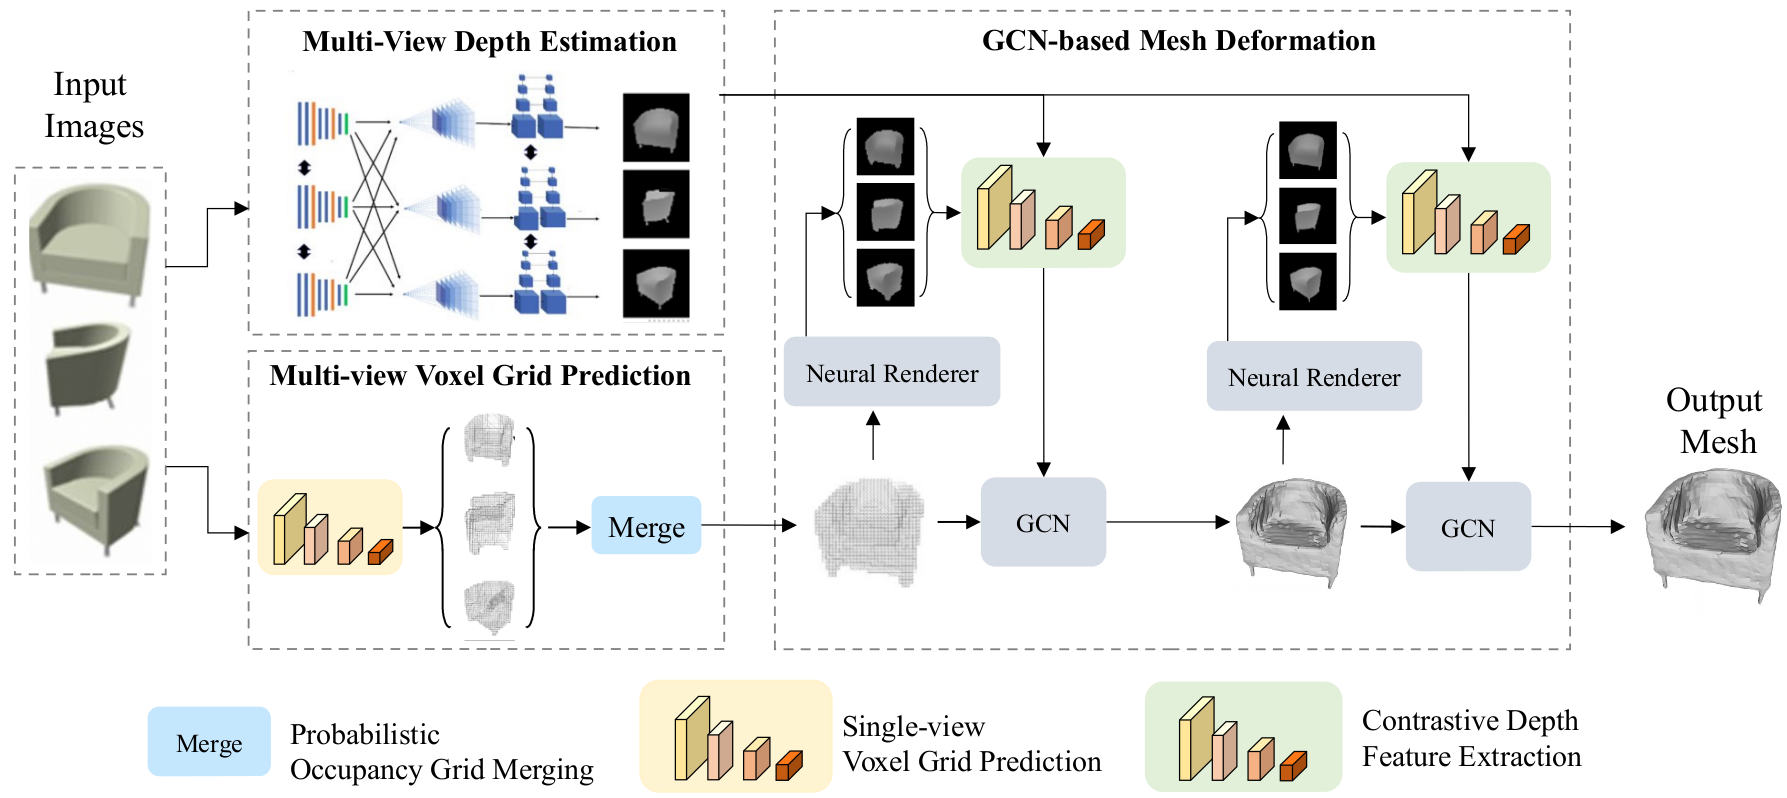
\includegraphics[width=0.95\linewidth]{imgs/arc.png}
\end{center}
\caption{
    \textbf{Architecture of the proposed method}.
    First, the voxel grid prediction module obtains a coarse voxel grid representation by probabilistically merging predicted voxel grids of each input image.
    Then, a series of GCNs further refine the cubified voxel grid in a coarse-to-fine manner using contrastive features from the rendered depths of the current shape and the depths from multi-view stereo.
    Specifically, the multi-view features are pooled using a attention-based mechanism.
}
\label{fig:system_architecture}
\end{figure*}

\paragraph{Single-view Shape Generation.}\vspace{-4mm}
Traditional single-view shape generation methods like~\cite{durou2008numerical,zhang1999shape,favaro2005geometric} reason about shading, texture and defocus to reason about visible parts of the object and infer its 3D geometry.
Earlier learning-based approaches~\cite{huang2015single, su2014estimating} use shape component retrieval and deformation from a large dataset for single-view 3D shape generation.
\cite{kurenkov2018deformnet} extend this idea by introducing free-form deformation networks on retrieved object templates from a database.
Some work learn shape deformation from ground truth foreground masks of 2D images~\cite{kar2015category,yan2016perspective,tulsiani2017multi}.
\cite{3dr2n2,hane2017hierarchical,johnston2017scaling} can learning 3D volumetric representations through deep learning.
Predicting 3D mesh from single-view color images has been proposed in~\cite{wang2018pixel2mesh,pan2019deep,gkioxari2019meshrcnn, tang2019skeleton}.
DR-KFS~\cite{jin2019drkfs} introduces a differentiable visual similarity metric to learn single-view 3D shape generation
while SeqXY2SeqZ~\cite{han2020seqxy2seqz} represents 3D shapes using a set of 2D voxel tubes for shape reconstruction.
Front2Back~\cite{yao2020front2back} generates 3D shapes by fusing predicted depth and normal images and
DV-Net~\cite{jia2020dv} predicts dense object point clouds using dual-view RGB images with a gated control network to fuse point clouds from the two views.
FoldingNet~\cite{yang2018foldingnet} learns to reconstruct arbitrary point clouds from a single 2D grid.
AtlasNet~\cite{groueix2018papier} use learned parametric representation
while \cite{mescheder2019occupancy,park2019deepsdf,liu2019learning,liu2019dist,murez2020atlas} employ implicit surface representation to reconstruct 3D shapes.

\paragraph{Multi-view Shape Generation.}\vspace{-4mm}
Multi-view 3D model generation has traditionally been tackled using stereo geometry principles.
Among them, structure-from-motion (SfM)~\cite{schonberger2016structure,agarwal2011building,cui2015global,cui2017hsfm} and simultaneous localization and mapping (SLAM)~\cite{cadena2016pastslam,mur2015orb,engel2014lsd,whelan2015elasticfusion} are popular techniques that perform 3D reconstruction and camera pose estimation at the same time.
% Closer to our problem setup, multi-view stereo methods infer 3D geometry from images with known camera parameters.
% These generally fall into one of two categories: Volumetric and Point Cloud based methods.
Similarly, traditional multi-view stereo methods infer 3D geometry from images with known camera parameters either using
volumetric representation~\cite{kutulakos2000theory, seitz1999photorealistic} or
point cloud representation~\cite{furukawa2009accurate, lhuillier2005quasi}.
These methods extract local image features, match them across images and use the matches to estimate 3D geometry.
While the results of these works are impressive in terms of quality and completeness of reconstruction, they still struggle with poorly textured and reflective surfaces and require carefully selected input views.

Deep learning based approaches can learn to infer 3D structure from training data and can be robust against poorly textured and reflective surfaces as well as limited and arbitrarily selected input views.
\cite{hartmann2017learned_16,deepmvs2018,yao2018mvsnet,chen2019point,luo2019pmvsnet,gu2019cascade,yao2019recurrent} propose multi-view stereo models from learned cost volumes to predict depth images.
Recurrent Neural Networks (RNN) based methods~\cite{3dr2n2, kar2017lsm, mcrecon2017} are another popular solution to solve this problem.
\cite{mcrecon2017, lin2019photometric} introduce image silhouettes along with adversarial multi-view constraints and optimize object mesh models using multi-view photometric constraints.
Pixel2Mesh++~\cite{wen2019pixel2mesh++} extends single-view Pixel2Mesh~\cite{wang2018pixel2mesh} to multi-view image input by introducing cross-view perceptual feature pooling and multi-view deformation reasoning but struggles to reconstruct complex shape topology due to its use of ellipsoidal template shape which it deforms to the final shape.
Our work avoids this pitfall by first predicting a coarse volumetric model which can represent complex topology and then applying deformations on it to get a finer shape as the final model.

% Pixel2Mesh~\cite{wang2018pixel2mesh} utilizes a single image of an object to predict its triangle mesh using perceptual features extracted from the image as GCN input.
% Voxel2Mesh~\cite{wickramasinghe2019voxel2mesh} extends Pixel2Mesh by using 3D volumes as input instead of 2D images.
% Pan et al.~\cite{pan2019deep} propose a similar progressive framework which alternates between neural networks for mesh deformation and topology modification for pruning error-prone faces.
% DR-KFS~\cite{jin2019drkfs} introduces a differentiable visual similarity metric for improving reconstruction quality of various shape generation methods.
% SeqXY2SeqZ~\cite{han2020seqxy2seqz} represent 3D shapes using a set of 2D voxel tubes which are predicted using RNN with a single image as input.
% Front2Back~\cite{yao2020front2back} generate 3D shapes by fusing predicted depth and normal images using Screen Poisson surface reconstruction~\cite{kazhdan2013screened}.
% Mesh R-CNN~\cite{gkioxari2019meshrcnn} utilizes instance segmentation to predict a coarse voxel grid which is further refined using GCNs to obtain a mesh from a single image.
% \cite{tang2019skeleton} further break down shape generation into skeleton prediction followed by voxel grid generation and finally GCN based mesh refinement.

% Recurrent Neural Networks (RNN) have been a popular solution for multi-view 3D reconstruction.
% 3D-R2N2~\cite{3dr2n2} employs 3D RNN with encoder-decoder architecture
% while LSM~\cite{kar2017lsm} uses recurrent 3D features grid fusion to predict 3D occupancy grid models.
% Gwak et al.~\cite{mcrecon2017} use image silhouettes along with adversarial multi-view constraints to estimate 3D voxel grid models.
% \cite{lin2019photometric} optimizes object mesh models using multi-view photometric constraint by piecewise image alignment of each mesh faces' rasterized projections.
% Pixel2Mesh++~\cite{wen2019pixel2mesh++} uses feature statistics from multi-view images to refine the mesh generated by Pixel2Mesh by further deforming the mesh vertices within a local neighborhood.

% We refer our readers to a recent survey on Deep Geometry Learning ~\cite{xiao2020survey} for a more comprehensive review of the related work on this topic.

% \paragraph{Depth Estimation}
% Compared to 3D shape generation, depth prediction is an easier problem formulation since it simplifies the task to per-view depth map estimation.
% Traditional methods ~\cite{campbell2008using,galliani2015massively,schonberger2016pixelwise} use multi-view stereo principles for depth prediction.
% Deep learning based multi-view stereo depth estimation was first introduced in~\cite{hartmann2017learned_16} where a learned cost metric is used to estimate patch similarities.
% DeepMVS~\cite{deepmvs2018} warps multi-view images to 3D space and then applies deep networks for regularization and aggregation to estimate depth images.
% Learned 3D cost volume based depth prediction was proposed in MVSNet~\cite{yao2018mvsnet} where a 3 dimensional cost volume is built using homographically warped 2D features from multi-view images and 3D CNNs are used for cost regularization and depth regression.
% This idea was further extended by~\cite{chen2019point,luo2019pmvsnet, gu2019cascade,yao2019recurrent}.

% Our system aims to combine the strengths of GCN based methods and depth prediction methods to improve the accuracy of the 3D structure while still ensuring completeness.
